% !Mode:: "TeX:UTF-8" 



\BiSection{2.13}{Figures}

\fancyhead[R]{本题2.13由QC.Z完成}



解:

\scalebox{3}{(a)}

MOS器件电容电路如图1所示

		\begin{figure}[H] %H为当前位置,!htb为忽略美学标准,htbp为浮动图形
	\begin{minipage}{\linewidth}
		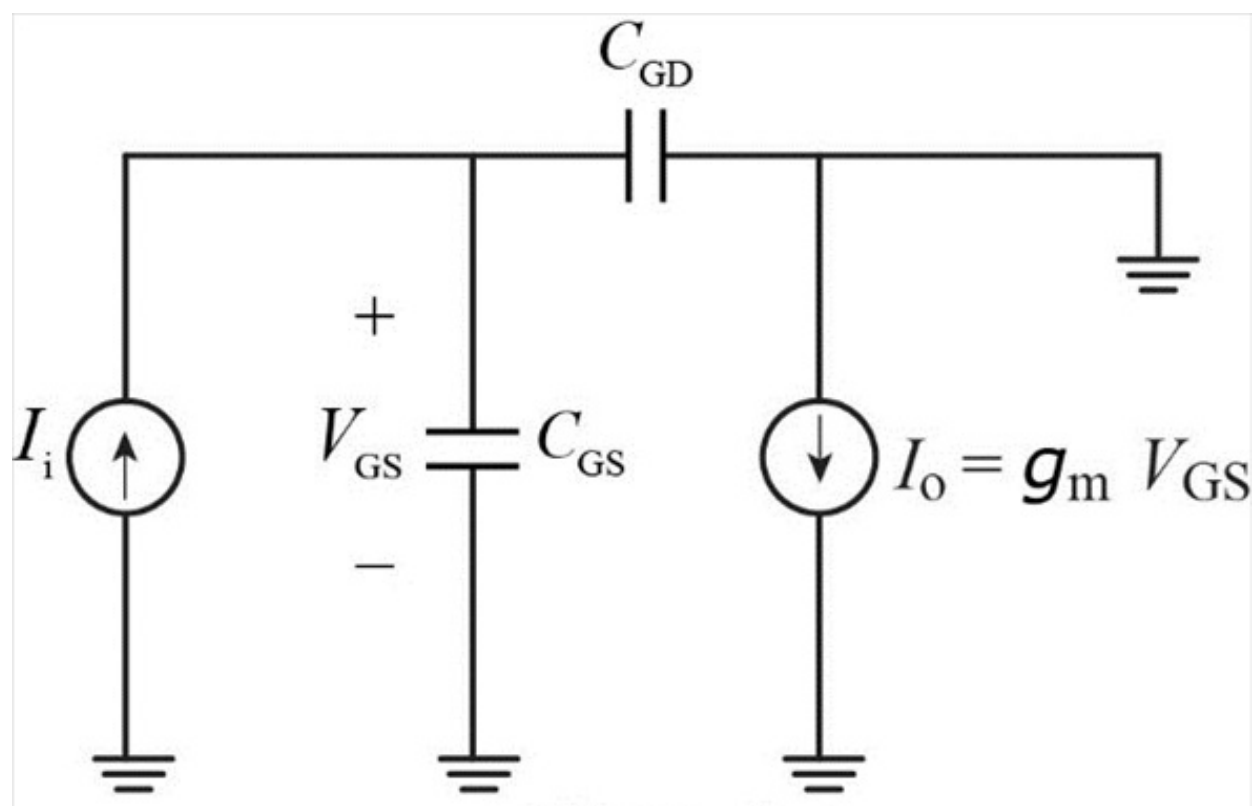
\includegraphics[width=1\linewidth]{2.13-1}
	\end{minipage}
	\caption*{图1} %最终文档中希望显示的图片标题
\end{figure}

在$V_{GS}$点用基尔霍夫电流定律Kirchhoff’s Current Law(KCL),有

	\begin{figure}[H] %H为当前位置,!htb为忽略美学标准,htbp为浮动图形
	\begin{minipage}{\linewidth}
		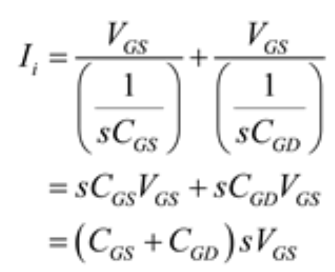
\includegraphics{2.13-2}
	\end{minipage}
\end{figure}

其中s是复参数‌,$C_{GD}$是每单位宽度栅漏电容,$C_{GS}$是每单位宽度栅源电容\textcolor{blue}{(因为方便计算等原因用复数容抗计算)}

小信号电流增益$\beta =\frac{I_o}{I_i}$


\begin{figure}[H] %H为当前位置,!htb为忽略美学标准,htbp为浮动图形
	\begin{minipage}{\linewidth}
		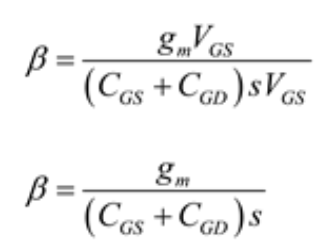
\includegraphics{2.13-3}
	\end{minipage}
\end{figure}

复平面$s=j {\omega}_r$。其中${\omega}_r$是特征角频率\textcolor{blue}{(transit angular frequency相当于每秒在单位圆上转过了多少弧度)}


\begin{figure}[H] %H为当前位置,!htb为忽略美学标准,htbp为浮动图形
	\begin{minipage}{\linewidth}
		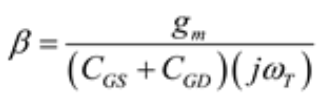
\includegraphics{2.13-4}
	\end{minipage}
\end{figure}

$|\beta |=1$


\begin{figure}[H] %H为当前位置,!htb为忽略美学标准,htbp为浮动图形
	\begin{minipage}{\linewidth}
		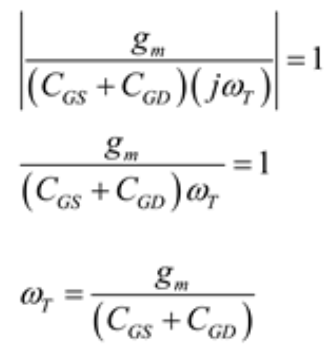
\includegraphics{2.13-5}
	\end{minipage}
\end{figure}

${\omega}_r=2\pi f_T$。其中$f_T$是特征频率\textcolor{blue}{(transit frequency相当于每秒在单位圆上转了$f_T$圈,$f_T=\frac{1}{T}$)}

\begin{figure}[H] %H为当前位置,!htb为忽略美学标准,htbp为浮动图形
	\begin{minipage}{\linewidth}
		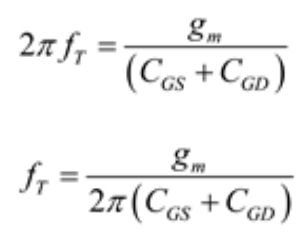
\includegraphics{2.13-6}
	\end{minipage}
\end{figure}

\scalebox{3}{(b)}

图2为器件等效为n个晶体管排列的示意图


\begin{figure}[H] %H为当前位置,!htb为忽略美学标准,htbp为浮动图形
	\begin{minipage}{\linewidth}
		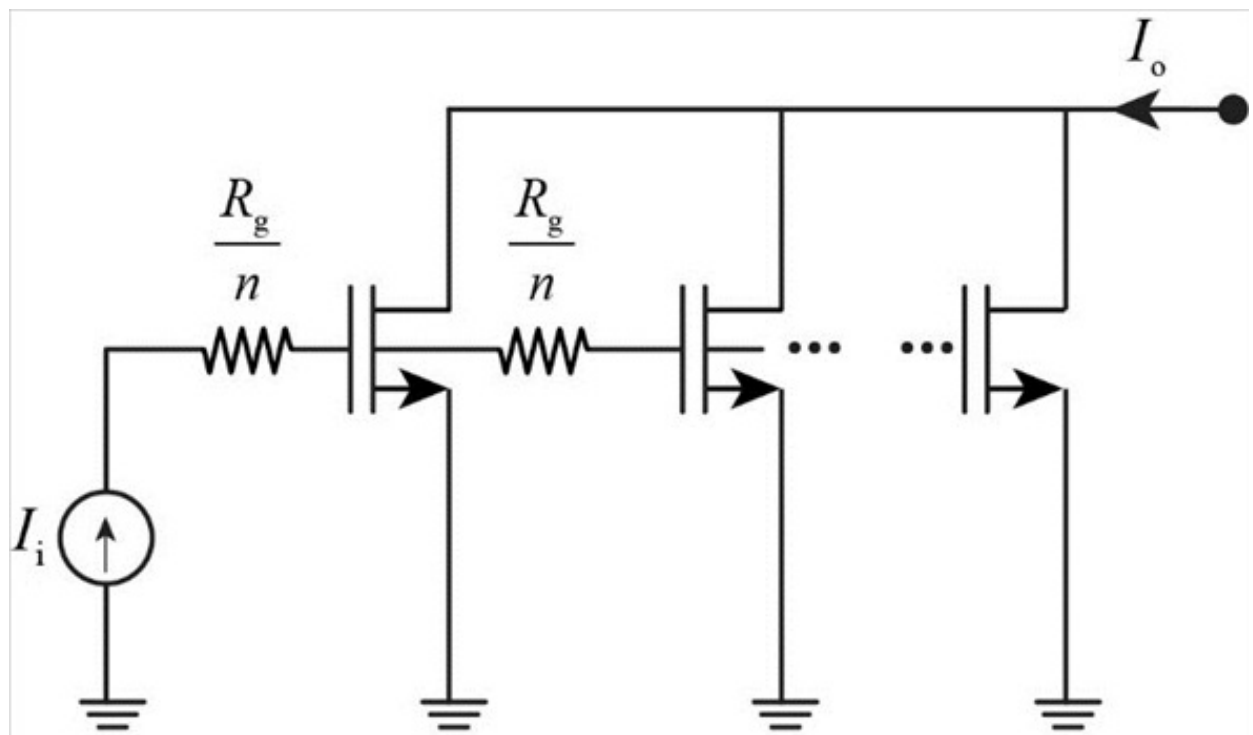
\includegraphics[width=1\linewidth]{2.13-7}
	\end{minipage}
	\caption*{图2} %最终文档中希望显示的图片标题
\end{figure}

图3为小信号等效电路图

\begin{figure}[H] %H为当前位置,!htb为忽略美学标准,htbp为浮动图形
	\begin{minipage}{\linewidth}
		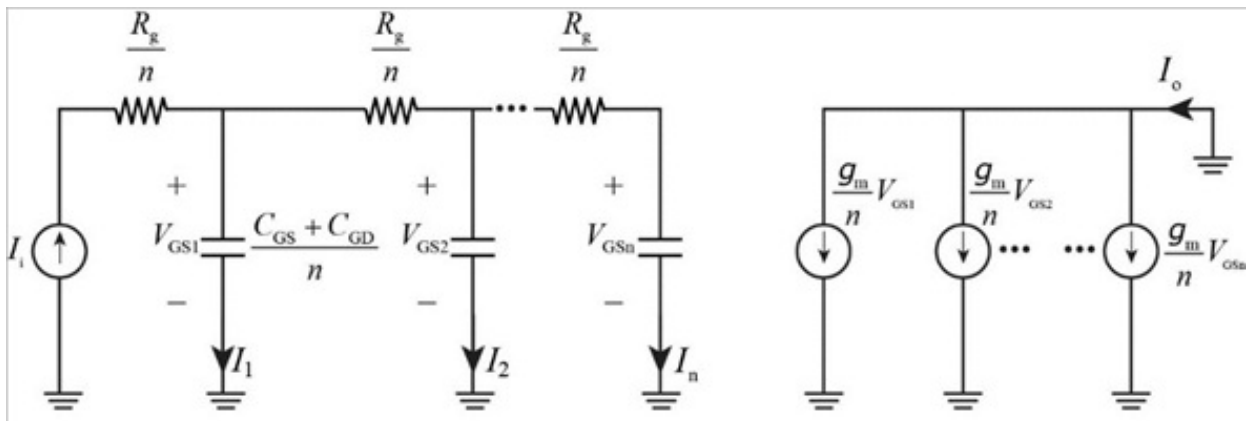
\includegraphics[width=1\linewidth]{2.13-8}
	\end{minipage}
	\caption*{图3} %最终文档中希望显示的图片标题
\end{figure}

$I_i=\frac{1}{n}(C_{GS}+C_{GD})sV_{GSk}.i,k=1,2,3...,n$

在图3用基尔霍夫电流定律Kirchhoff’s Current Law(KCL),有

\begin{figure}[H] %H为当前位置,!htb为忽略美学标准,htbp为浮动图形
	\begin{minipage}{\linewidth}
		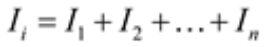
\includegraphics{2.13-9}
	\end{minipage}
\end{figure}

\begin{figure}[H] %H为当前位置,!htb为忽略美学标准,htbp为浮动图形
	\begin{minipage}{\linewidth}
		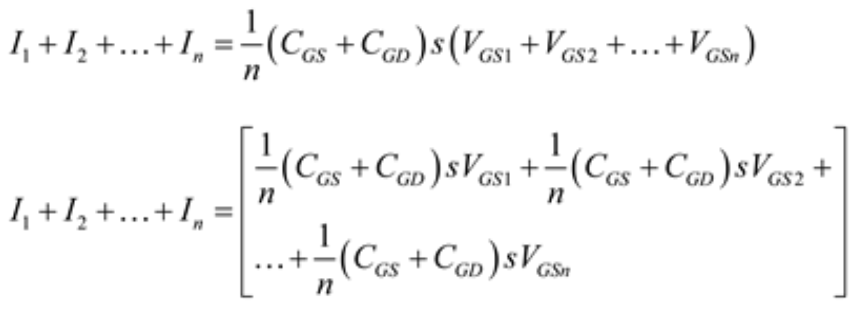
\includegraphics{2.13-10}
	\end{minipage}
\end{figure}

\begin{figure}[H] %H为当前位置,!htb为忽略美学标准,htbp为浮动图形
	\begin{minipage}{\linewidth}
		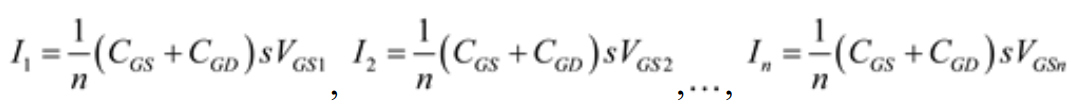
\includegraphics[width=1\linewidth]{2.13-11}
	\end{minipage}
\end{figure}









\begin{figure}[H] %H为当前位置,!htb为忽略美学标准,htbp为浮动图形
	\begin{minipage}{\linewidth}
		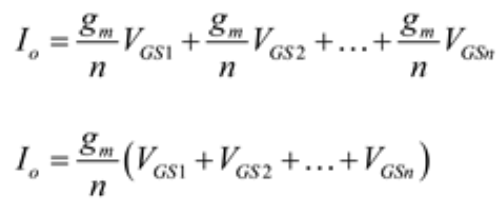
\includegraphics{2.13-12}
	\end{minipage}
\end{figure}

考虑上式第一项,有

\begin{figure}[H] %H为当前位置,!htb为忽略美学标准,htbp为浮动图形
	\begin{minipage}{\linewidth}
		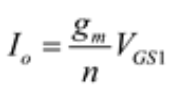
\includegraphics{2.13-13}
	\end{minipage}
\end{figure}

小信号电流增益$\beta =\frac{I_o}{I_i}$

\begin{figure}[H] %H为当前位置,!htb为忽略美学标准,htbp为浮动图形
	\begin{minipage}{\linewidth}
		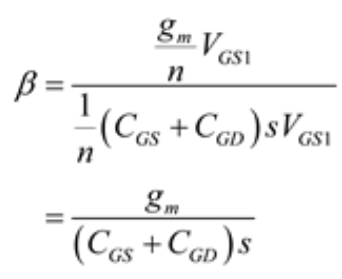
\includegraphics{2.13-14}
	\end{minipage}
\end{figure}

\begin{figure}[H] %H为当前位置,!htb为忽略美学标准,htbp为浮动图形
	\begin{minipage}{\linewidth}
		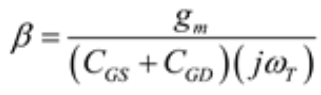
\includegraphics{2.13-15}
	\end{minipage}
\end{figure}

$|\beta |=1$


\begin{figure}[H] %H为当前位置,!htb为忽略美学标准,htbp为浮动图形
	\begin{minipage}{\linewidth}
		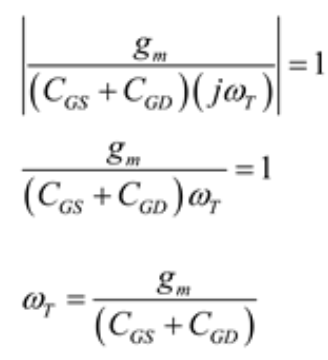
\includegraphics{2.13-16}
	\end{minipage}
\end{figure}

\begin{figure}[H] %H为当前位置,!htb为忽略美学标准,htbp为浮动图形
	\begin{minipage}{\linewidth}
		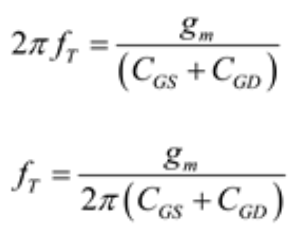
\includegraphics{2.13-17}
	\end{minipage}
\end{figure}

\scalebox{3}{(c)}

$g_m=\mu_nC_{ox}\frac{W}{L}(V_{GS}-V_{TH})$\textcolor{blue}{(P18的2.18)}

平行板电容器$C_{GS}$和$C_{GD}$的总电容约等于$C_{ox}WL$,因此$C_{GS}+C_{GD}\cong C_{ox}WL$.其中$C_{ox}$是每单位区域栅氧电容


\begin{figure}[H] %H为当前位置,!htb为忽略美学标准,htbp为浮动图形
	\begin{minipage}{\linewidth}
		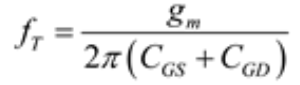
\includegraphics{2.13-18}
	\end{minipage}
\end{figure}

\begin{figure}[H] %H为当前位置,!htb为忽略美学标准,htbp为浮动图形
	\begin{minipage}{\linewidth}
		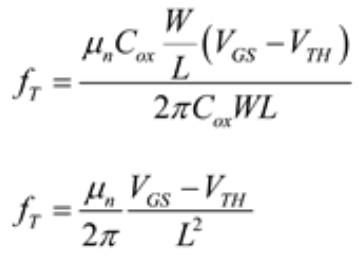
\includegraphics{2.13-19}
	\end{minipage}
\end{figure}



